\chapter{Work Overview}

Two main branches can be identified in the algorithms developed for the terrain coverage: online and offline search methods. This two branches can fit different needs, that are related to the type of hardware to which are applied to, i.e. micro-robots swarm or advanced-robots swarm. In particular online search is a better choice for micro-robots that have restricted computational capability since they only have to perform a search on adjacent cells and make simple comparison choices. The optimisation algorithms implemented instead require a discrete computational capability since they analyse all the graph and compute many the possible combinations before taking the choice.

\noindent In this thesis work the following methods have been investigated:

\begin{itemize}
\item Online Algorithms
	\begin{enumerate}
	\item Node Counting	
	\item Learning Real-Time A*
	\item Edge Counting
	\item PatrolGRAPH*
	\end{enumerate}

\item Offline Algorithms
	\begin{enumerate}
	\item VRP Greedy Nearest Neighbour
	\item VRP Greedy A*
	\item VRP Greedy with Floyd-Warshall
	\end{enumerate}
\end{itemize}
From now on, for convenience, we will refer to the Learning Real-Time A* as LRTA*, and in the VRP Greedy we will frequently omit the \emph{greedy} attribute.

The way the algorithms operate allow to classify them also in two other classes: \emph{distributed} and \emph{centralised} algorithms. In fact, while in the real-time algorithms the quadcopters are autonomous and compute their paths while moving, the optimised algorithm require a central brain that calculates the optimal paths and send them to the quadcopters. Nevertheless a distributed version of the optimised algorithm is possible to implement by distributing the evaluation of the algorithm among the robots.
In the next two chapters both types of algorithms will be discussed in depth, providing a detailed explanation, pseudo-code of the algorithm, images of the generated ROS graph network and sample screen-shots of the simulator at the end of the coverage (trails are left by the quadcopters while moving).

\begin{figure}[H]
\centering
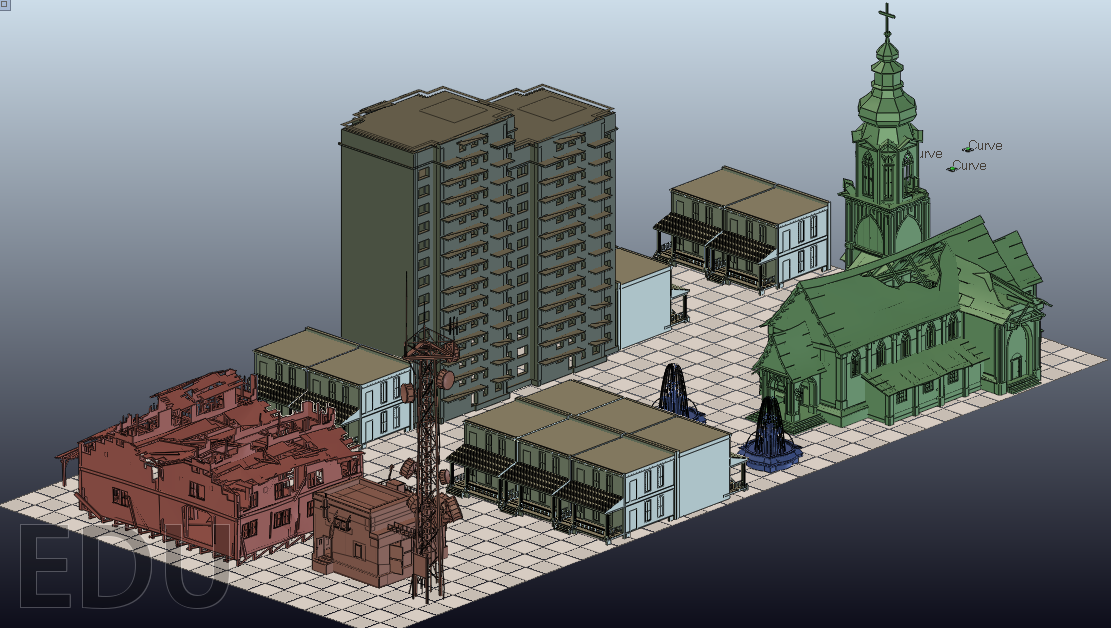
\includegraphics[width=\textwidth]{simulation_environment}
\caption{The 3D simulation environment}
\label{fig:simEnv}
\end{figure}


To test the algorithms the 3D simulation environment was created from scratch using the VREP robotic simulator (Fig. \ref{fig:simEnv}). The map has been created trying to include a variety of topology characteristics, such as: dead ends, loops and open-spaces.
As stated in the first chapter the environment map is sub-sampled using a regular grid, and a binary value is assigned to every cell of the grid: \textbf{0} represent an accessible cell, while \textbf{1} represents an occupied cell, as shown in Fig. \ref{fig:mapGrid}.  There exists a vertex $v \in V$ for every cell of the grid, and every vertex $v$ is connected to its accessible adjacent $w_i$ vertices with an undirected edge $e=(v,w_i) \in E$. The result, is a strongly connected graph, where every node $v$ can be reached from every vertex $w$ directly, or by traversing a finite number of vertices. The edge cost is simply calculated using the euclidean distance. The edge connecting two neighbours has always the same cost. Nevertheless a possible extension can be applied in the search methods using the A* path finding algorithm \cite{4082128}. The matrix used by the A* in fact is not binary. To an accessible cell instead, a value from 0 to 5 can be assigned, which represents the cost of travelling across that particular cell. Zero means the least possible difficulty in travelling whilst five represents the most difficult, .


%\begin{figure}[H]
%\centering
%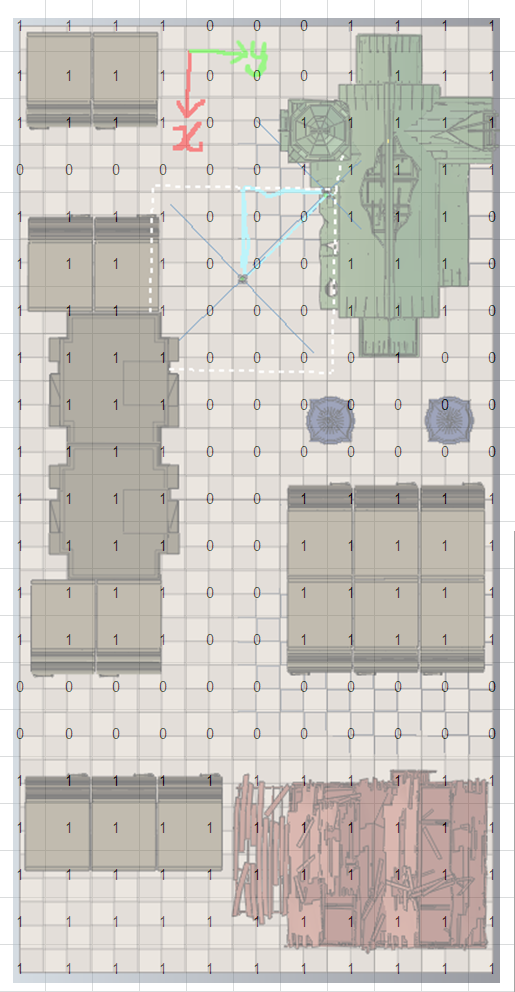
\includegraphics[scale=0.4]{map_grid}
%\caption{The binary access matrix built on top of the 3D environment}
%\label{fig:mapGrid}
%\end{figure}

\begin{figure}[H]
  \begin{minipage}[b]{0.45\linewidth}
    \centering
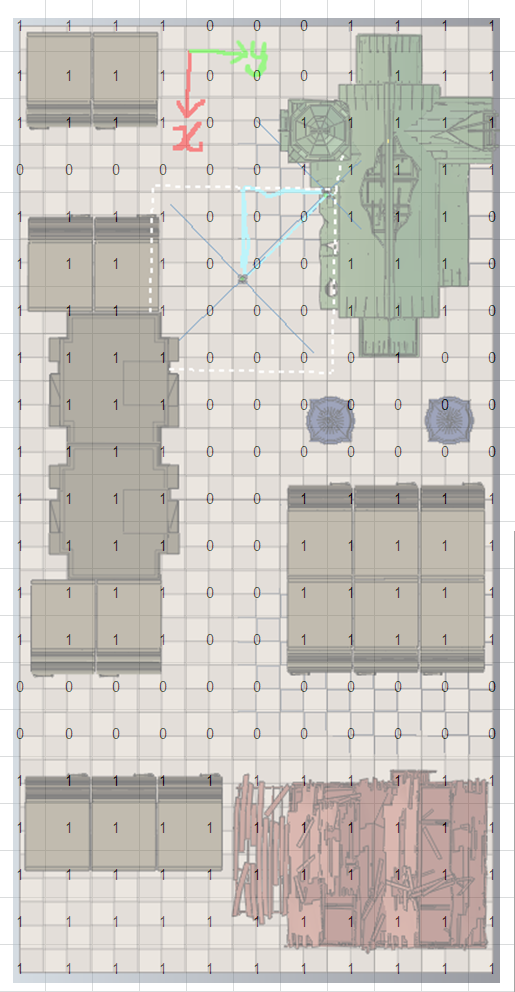
\includegraphics[scale=0.4]{map_grid}
\caption{The binary access matrix built on top of the 3D environment}
\label{fig:mapGrid}
    %\vspace{4ex}
  \end{minipage}
\quad
  \begin{minipage}[b]{0.45\linewidth}
    \centering
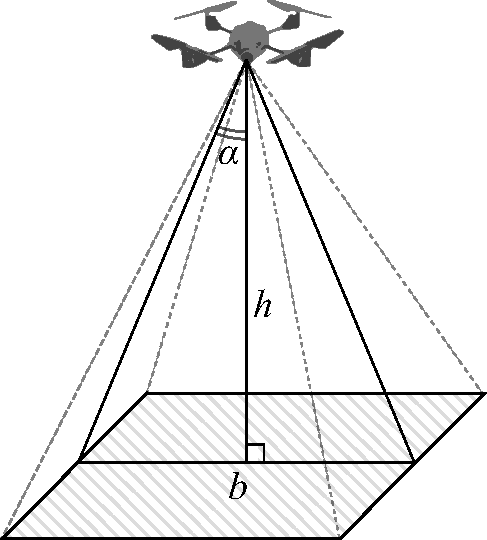
\includegraphics[scale=0.7]{quad_fov}
\caption{Scheme for the calculation of the view surface}
\label{fig:quadFov}
   % \vspace{4ex}
  \end{minipage}
\end{figure}

From Fig. \ref{fig:quadFov} we can see that, using downward facing cameras with a square vision sensor having a view angle of $2\alpha$ mounted on the hovering robot flying at height $h$, the side $b$ of the projected square that defines the view surface can be calculated as:
\begin{equation}
b = 2(h \tan(\alpha))
\label{eq:viewSide}
\end{equation}
So following formula \ref{eq:viewSide} we can set the flying height $h$ such that a cell, of side $b$, is completely covered. 
The input of the coverage solver is then a simple text file containing the occupancy grid matrix. The coverage planner will store the vertices of the graph as a vector of structs (C++ standard template library) associating the \emph{position}, \emph{occupancy} and \emph{visit count} properties as in Fig. \ref{fig:graph_struct}, and a separate adjacency graph so to apply all the discussed algorithms. In this way it's really easy to describe a terrain so that having for example just an image of a geographic area we can easily convert it to an occupancy grid using some dedicated software manually or automatically. We can observe anyway that not-accessible cells of the map will never be taken into account by the algorithm since no edge points to them, but they will still occupy memory space. That's why an alternative input method has been provided for the controllers, consisting in a map already represented as an adjacency graph but containing only the accessible vertices, with an auxiliary file specifying the position in the space for each vertex. Using this representation of course the process of converting a raw image to a consistent graph becomes a little bit more complex and for small maps the reading time and memory allocation space may not vary significantly, but with bigger and more detailed maps the advantages may become considerable. The grids in Fig. \ref{fig:grid1} and Fig. \ref{fig:grid2} for example are represented using adjacency graphs.

\begin{figure}[H]
\centering
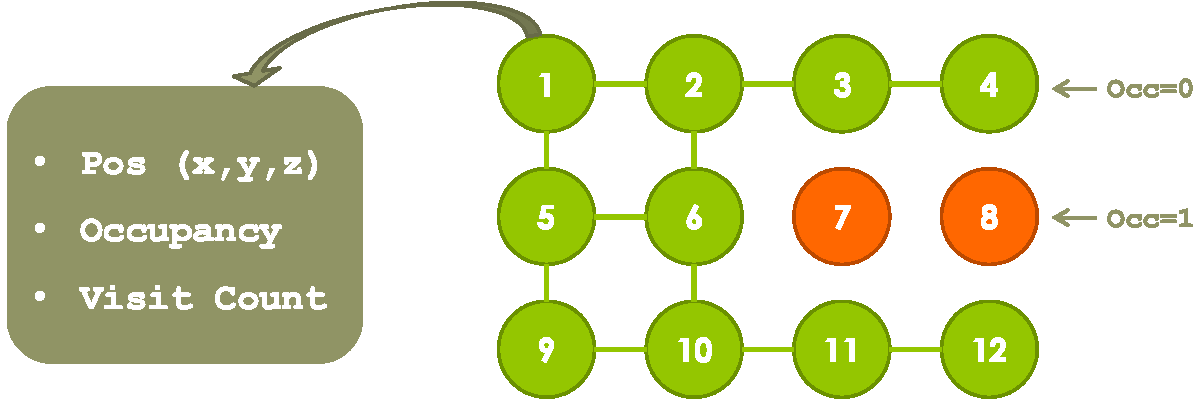
\includegraphics[scale=0.6]{graph_structure}
\caption{Graph structure}
\label{fig:graph_struct}
\end{figure}

\section{The way-point planning algorithm}

The basic mechanism used to move the quadcopters relies on the fact that in the simulator, to each quadcopter is associated a so called manipulating sphere, shortly the MP, which the quadcopter follows whenever the sphere centre does not coincide with its centre. It comes natural then to understand that the \emph{quad} controllers move this spheres to manipulate the robots in the environment. 
While performing the coverage the quadcopters move only from one vertex to a neighbour one and, under this condition no obstacle can be found if the map is accurate enough. Anyway a short remark has to be done about this: since the control algorithm embedded in the quadcopter of the V-REP simulator is (as stated by the algorithm's author) ``quickly written and is dirty and not optimal'', an additional path planning was developed beneath the search algorithms.
In particular if the MP is placed too far away, the thrust given to the propellers of the quadcopter, being directly proportional to the distance MP$\rightarrow$quadcopter, becomes too high. This causes the quadcopter to become highly unstable and eventually lose control and crash. To overcome this problem a `critical distance' has been defined, and if the MP$\rightarrow$quadcopter distance is greater then the critical one, intermediate way-points are dynamically interpolated to safely guide the quadcopter to the target.
So combining this necessity with the one of following a given path vertex by vertex, a waypoint follower algorithm was developed with the logic shown in Fig. \ref{fig:wp_flowch}.


\begin{figure}[t]
\centering
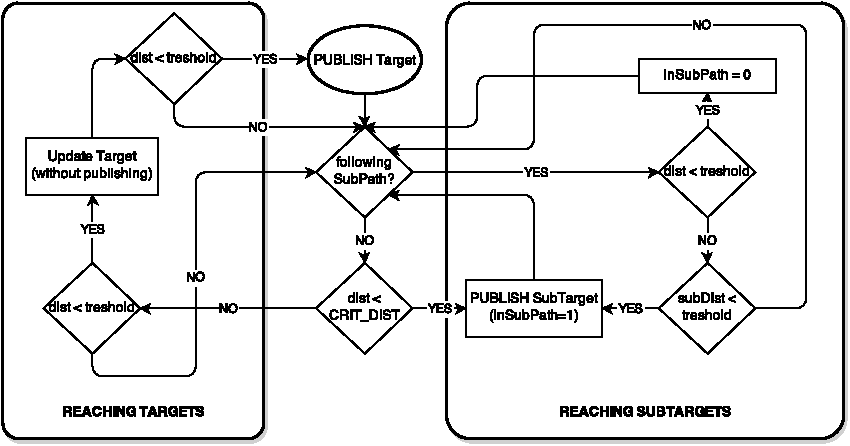
\includegraphics[width=\textwidth]{way-point_flowch}
\caption{The flow-chart of the inter-vertex trajectory planning}
\label{fig:wp_flowch}
\end{figure}

In the flow-chart the way-points relative to a vertex are called targets, while the \mbox{way-points} between two vertices are called sub-targets. The distance between a quadcopter and the target is called \textit{dist} while the distance between a quadcopter and a sub-target is called \textit{subDist}. The critical distance mentioned above is shortened as \textit{CRIT\_DIST}.
This argumentation does not apply to the control of the real quadcopter since the platform used for the experiments on the field. an Asctec\textsuperscript{TM} Pelican has a very good PID controller (better described further on) for which the targets are just sent without sub-path-planning.

All this control logic is contained within a bigger one where we check whether we acquired the quadcopter position (needed for all the distance comparisons) and if we have completed the coverage.
